%%%%%%%%
% Highlevel
% ca 1-2 Seiten
% Buzzwords, grober Überriss
% Hier wird erklärt, mit welchem Ansatz an das Projekt herangegangen wurde
\section{Lösungsansatz}

% Warum wurde sich für die Darstellung der Mandelbrotmenge entschieden
\subsection{Verwendung der Mandelbrotmenge}

Es handelt bei der Bestimmung der Mandelbrotmenge um eine rechenintensive Operation, wobei
die benötigte Zeit linear mit der maximalen Iterationszahl \( I_{max} \) skaliert.
Zusätzlich ist die Berechnung für jede einzelne komplexe Zahl \( c\in \mathbb{C} \)	unabhängig.

Daher ist eine einfache Parallelisierung mit den folgenden Eigenschaften möglich:
\begin{itemize}
	\item Die Rechendauer kann durch die maximale Iterationszahl \( I_{max} \) bestimmt werden.
	\item Durch die paarweise Unabhängigkeit der Punkte, können diese ohne Datenaustausch parallel berechnet werden.
\end{itemize}

Somit kann gesichert werden, dass die Benutzerin eine wahrnehmbare Zeit \( (100 - 200 ms) \) zur Berechnung der Punkte innerhalb
der Mandelbrotmenge erlebt.
Aus didaktischer Sicht ist dies wichtig, um Differenzen zwischen den Balancierungsstrategien spürbar zu machen.
Zudem kann die Unterteilung des zu berechnden Raumes frei gewählt werden, sodass
verschiedenste Aufteilungen möglich sind und insbesondere bei der Lastbalancierung frei eingeteilt werden kann.

Da das Projekt auch nicht technisch versierte Anwender durch die Ästhetik der Mandelbrotmenge anspricht, eignet es
sich, um ein erstes Interesse für Parallelisierung wecken.

% Wie wurde die Parallelisierung angegangen?

\subsection{Parallelisierung}

Die Parallelisierung soll auf drei verschiedene Weisen implementiert werden.

Das Hauptaugenmerk liegt auf der Parallelisierung mithilfe von MPI.
Dazu wird der zu berechnende Ausschnitt der Mandelbrotmenge in Teilregionen aufgeteilt
welche jeweils einem Rechenknoten ("Worker") per MPI zugewiesen werden.
Das Ergebnis der Berechnung wird wieder per MPI an den aufteilenden und verwaltenden Knoten ("Host")
zurückgesandt.

Außerdem kann die Berechnung mehrerer Pixel in einer Teilregion parallelisiert werden.
Dazu wird OpenMP auf die Schleife über die Pixel der Region angewandt.
OpenMP sorgt dann selbst dafür, dass die einzelnen Iterationen gleichmäßig auf die vorhandenen
Threads, einen pro Rechenkern, verteilt werden.
Das Ergebnis wird in eine geteilte Datenstruktur geschrieben.

Zuletzt wird die feinste Parallelisierung per SIMD angewandt.
Dazu wird die Berechnung von je 2 oder 4 Pixeln in 2 oder 4 SIMD-Lanes parallel durchgeführt.

% Wie ist die (grobe) Architektur des Programmes (parallelisiertes Backend, Oberfläche)
\subsection{Architekturübersicht}\label{sec:architektur}
\begin{figure}
	\centering
	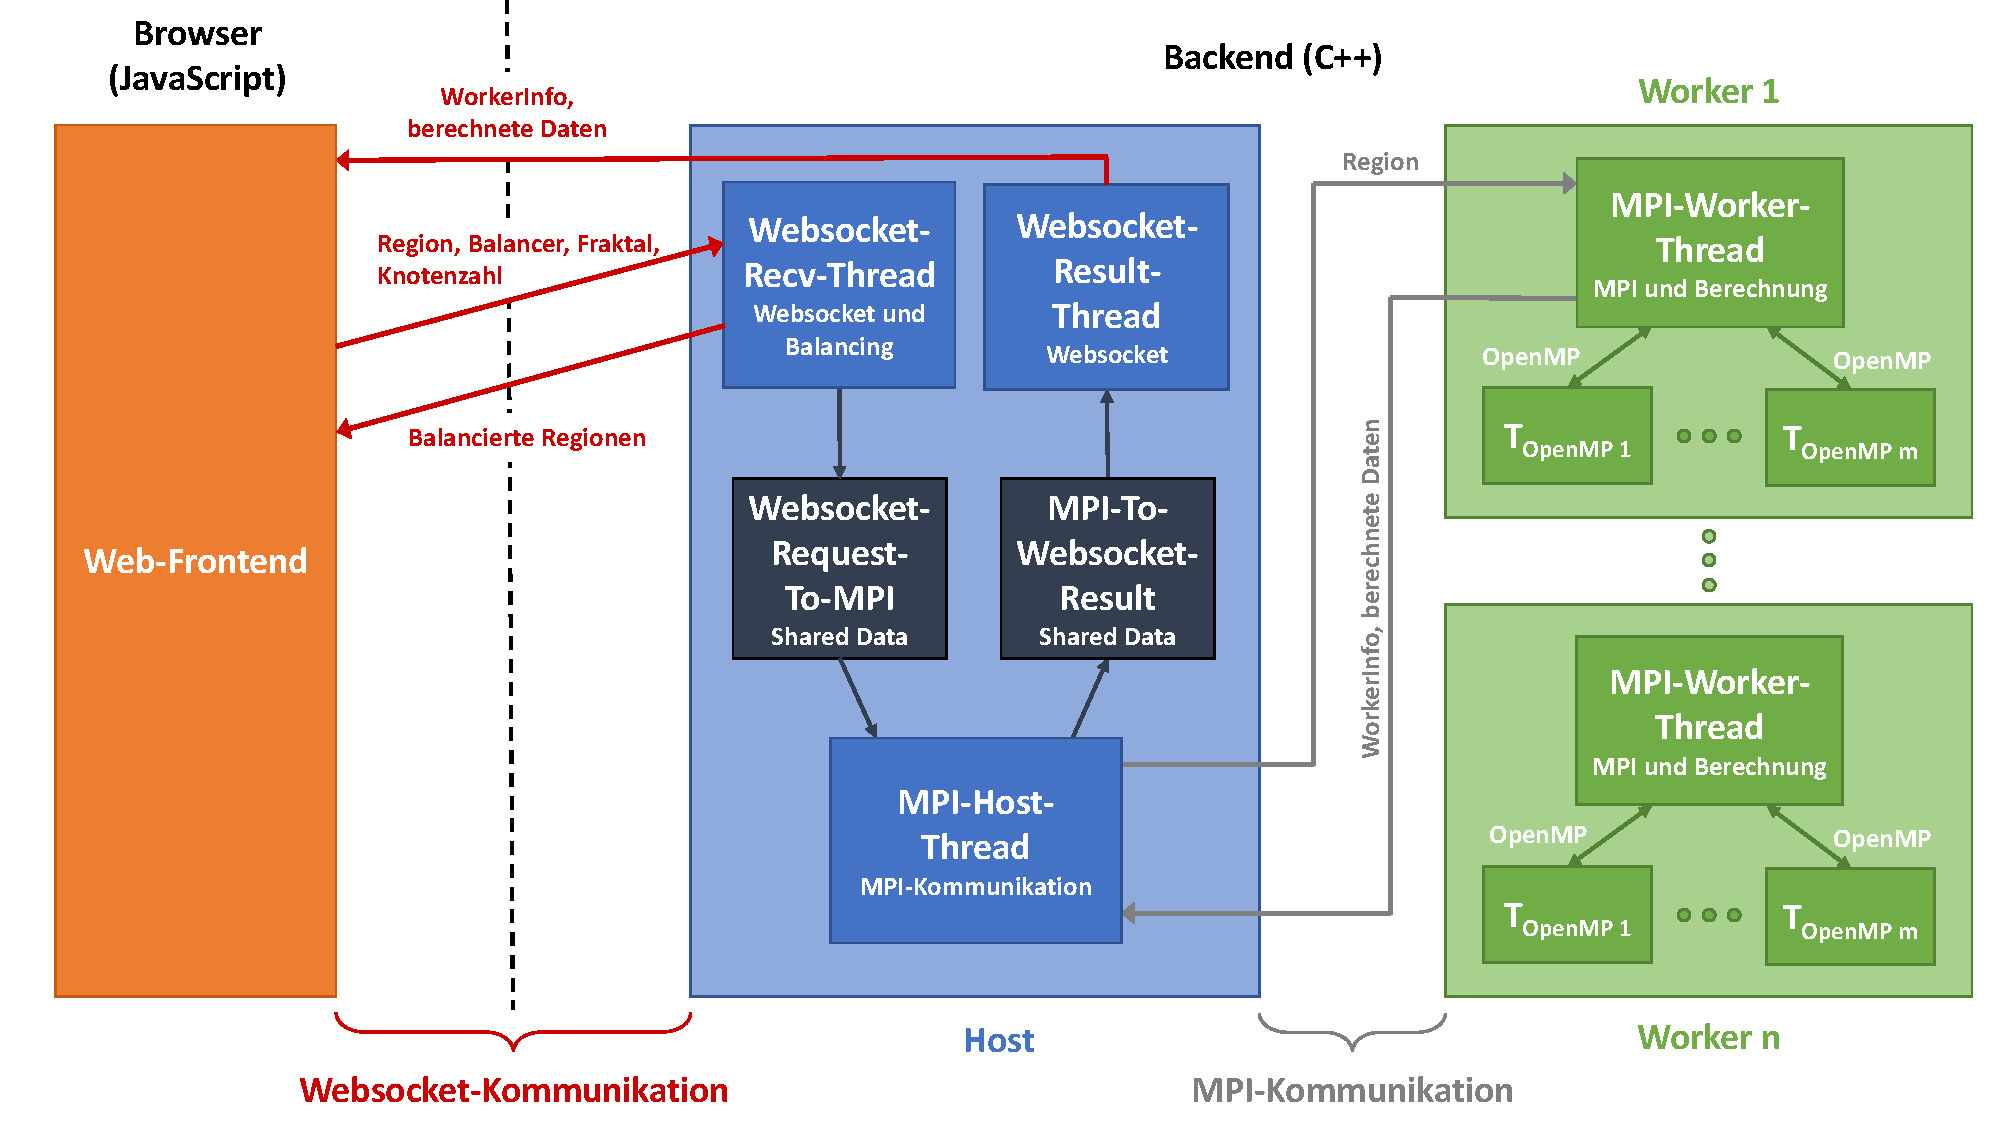
\includegraphics[width=\linewidth]{img/Implementierung/ArchitekturAusfuehrlich.pdf}
	\caption{Architekturübersicht}
	\label{fig:architekturuebersicht_detail}
\end{figure}

Die hohe Rechenintesivität erfordert, dass der Berechnungsteil des Projektes in einer
hardwarenahen Sprache umgesetzt wird.
Andererseits sollte die Benutzeroberfläche einfach zu bedienen und auf möglichst vielen verschiedenen Geräten lauffähig sein.
Daher wurde sich für eine Zweiteilung entschieden, in ein Frontend, im Browser aufrufbar, und ein Backend, auf einem Rechencluster
laufend und hardwarenah programmiert.

Die Gesamtarchitektur besteht aus drei wesentlichen Bausteinen, die in \autoref{fig:architekturuebersicht_detail} zu sehen sind:
\begin{itemize}
	\item Eine Benutzeroberfläche im Webbrowser (Frontend), die Benutzereingaben entgegennimmt und die Ergebnisse darstellt.
	\item Ein Backend-Host, der eingehende Rechenaufträge vom Frontend an die Worker verteilt und deren Ergebnisse an das Frontend weiterleitet.
	\item Mehrere Backend-Worker, die die eigentliche Berechnung parallel durchführen.
\end{itemize}

% Welche Lastbalancierungsmechanismen wurden umgesetzt?
\subsection{Lastbalancierung}\label{sec:load_balancing_concepts}
Um die Effizienz der parallelen Berechnung der Mandelbrotmenge zu erhöhen, sollte die Rechenlast möglichst gleichmäßig auf die Worker verteilt werden.
Die Aufgabe der Lastbalancierung besteht darin zu einer gegebenen Region und einer Anzahl von Workern eine solche Unterteilung in sogenannte Teilregionen zu finden.
Damit die Unterschiede zwischen guter und schlechter Lastverteilung deutlich werden, stehen in diesem Projekt verschiedene, dynamisch austauschbare Strategien der Lastbalancierung zur Wahl.

\paragraph{Naive Strategie}
Bei der naiven Strategie wird versucht den einzelnen Workern etwa gleich große Teilregionen zuzuweisen.
Dies geschieht allerdings ohne Beachtung der eventuell unterschiedlichen Rechenzeiten innerhalb der Teilregionen, was zu einer schlechten Lastverteilung führen kann.

\paragraph{Strategie mit Vorhersage}
Bei dieser Strategie basiert die Aufteilung der Region auf einer Vorhersage über die Rechenzeit.
Die Teilregionen werden so gewählt, dass sie, entsprechend der Vorhersage, etwa einen ähnlichen Rechenaufwand haben.
Die optimale Rechenlast für einen Worker berechnet sich also durch:

\begin{equation}\label{equ:desiredN}
	\frac{Gesamtrechenlast}{AnzahlWorker}
\end{equation}

Wenn die Vorhersage hinreichend exakt ist, kann dieser Wert gut angenähert werden.
Dadurch wird die Last gleichmäßiger auf die Worker verteilt als bei der naiven Strategie.

\paragraph*{Bestimmung der Vorhersage}\label{par:load_balancing_prediction}
Die Zugehörigkeit eines Punktes zur Mandelbrotmenge wird nach \autoref{equ:mandelbrot} iterativ berechnet.
Deshalb kann die Anzahl der benötigten Iterationen als Abschätzung der Rechenzeit für diesen Punkt verwendet werden.
Zur Anstellung der Vorhersage wird also die angeforderte Region in deutlich geringerer Auflösung berechnet.
Dies ist eine gute Annäherung an die tatsächlich Rechendauer, da benachbarte Punkte meist eine ähnliche Anzahl an Iterationen benötigen.
Einzig am Rand der Mandelbrotmenge kommt es zu Ungenauigkeiten, weil dort Punkte innnerhalb und außerhalb der Menge für die Vorhersage zusammenfallen.
Die Genauigkeit der Vorhersage zu erhöhen bedeutet zusätzlichen Rechenaufwand während der Balancierung.
Dieser sollte in einem sinnvollen Verhältnis zum Aufwand der Berechnung der Region selbst stehen.

\paragraph{Implementierungsvarianten}
Sowohl die naive Strategie als auch die Strategie mit Vorhersage lassen sich in zwei Varianten umsetzen.
Man kann einen ganzheitlichen oder einen rekursiven Ansatz wählen.
Bei ersterem wird die gesamte Region in einem Schritt in die gewünschte Anzahl an Teilregionen geteilt.
Dazu werden Zeilen und Spalten gebildet.
Die Grundidee eines rekursiven Ansatzes ist es das Problem so lange in einfachere Teilprobleme aufzuteilen, bis die Lösung offensichtlich ist (Basisfall).
Hier ist der Basisfall die Aufteilung einer Region auf genau einen Worker.
Um diesen zu erreichen wird die Region solange halbiert, bis genug Teilregionen für jeden Worker entstanden sind.

Wo die Grenzen zwischen den Zeilen und Spalten (nicht-rekursiv) bzw. den Hälften (rekursiv) liegen, wird von der zugrundeliegenden Lastbalancierungsstrategie bestimmt.

% Wie wurde die Kommunikation per MPI angegangen?
\subsection{Nachrichtenaustausch}
Um zwischen den unabhängigen Systemen eine einheitliche Kommunikation zu ermöglichen,
wurde ein Protokoll spezifiziert um Flächen in der komplexen Ebene und ihre Auflösung eindeutig zu bestimmen.
Der grobe Inhalt und die Richtung der Nachrichten ist \autoref{fig:architekturuebersicht_detail} zu entnehmen,
die exakte Spezifikation in der jeweiligen Sprache findet sich in den angegebenen Dateien.

% TODO: improve
\begin{figure}
	\centering
	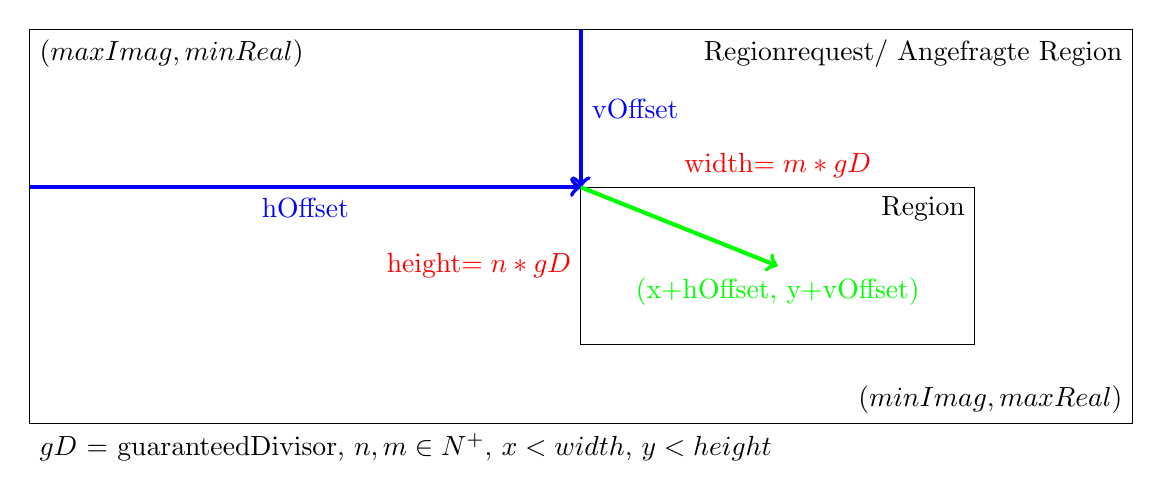
\begin{tikzpicture}[scale=1]
		% Superregion
		\draw (0,0) rectangle (14,5) node[below left] {Regionrequest/ Angefragte Region};
		% subregion
		\draw (7,1) rectangle (12,3) node[below left] {Region};
		% width height
		\draw (7,3) -- node[above, red] {width$=m*gD$} (12,3);
		\draw (7,1) -- node[left, red] {height$=n*gD$} (7,3);
		% vOffset/hOffset
		\draw[blue, ->, line width=1.5pt] (7,5) -- (7,3) node[midway, anchor=west] {vOffset};
		\draw[blue, ->, line width=1.5pt] (0,3) -- (7,3) node[midway, anchor=north] {hOffset};
		% x/y
		\draw[green, ->, line width=1.5pt] (7,3) -- (9.5,2) node[below] {(x+hOffset, y+vOffset)};
        \draw (0, 0) node[below right] {$gD$ = guaranteedDivisor, $n,m \in \mathbb{N}^{+}$, $x < width$, $y < height$};
        \draw (14,0) node[above left] {$(minImag, maxReal)$};
        \draw (0,5) node[below right] {$(maxImag, minReal)$};
	\end{tikzpicture}
	\caption{Konzept der Kooridinaten in den Regionsobjekten. Alle Koordinaten beziehen sich auf die Darstellungsebene und sind daher in Pixeln.}
	\label{fig:concept_coordinates}
\end{figure}

Bei einer Anfrage wird eine Region in komplexen Koordinaten beschrieben, wobei der obere linke Punkt $(maxImag, minReal)$
und der rechte untere Punkt $(minImag, maxReal)$ in der komplexen Ebene einen zu berechnenden Bereich aufspannen.
Da die reelle Ebene jedoch beliebig genau aufgelöst werden kann, muss zudem noch die Anzahl an Pixeln
pro Seite des Rechteckes definiert werden, \verb|width| und \verb|height|.
Wie in \autoref{fig:concept_coordinates} zu sehen, ist zudem der horizontale Offset und vertikale Offset
die linke obere Koordinate der Region bezüglich der gesamten sichtbaren Anfrage in Pixeln (diese Werte
gewinnen in den Regionsaufteilungen an Bedeutung).

In zurückkehrenden \verb|RegionData|-Nachrichten sind Arrays der berechneten Iterationszahlen eingebunden.
Dabei wird der Punkt (x, y) in der gesendeten Region (Punkt (x+hOffset, y+vOffset) in der angefragten Region)
im Datenarray an Index $i = x + y * width$ gespeichert.
